\section{Experiments}
%each part
%connections btw parts



\subsection{The paths to a compressed language model}\label{sec:3path}

% Unlike the previous section which describes \textit{how} to compress, this section describes \textit{when} to compress. 

This section describes how we obtain a compressed model under the popular pre-training schemes of language models. Figure \ref{fig:scheme} illustrates three paths that we examined for creating compressed language models. All the paths start from retraining a large transformer-based model pre-trained with a large language corpus in a self-supervised way, called the generic pre-training ($L \rightarrow L^g$). 

The path-1 ($S \rightarrow S^g \rightarrow S^t$) is a popular scheme that creates a small model first, then performs the generic distillation for the small model to learn the knowledge of the large model. The resulting small generic model $S^g$ will be fine-tuned with the target task dataset to obtain the task-specific model $S^t$. The representative works of path-1 include DistilBERT \citep{sanh2019distilbert}, TinyBERT \citep{jiao2019tinybert}, MobileBERT \citep{sun2020mobilebert}, and MiniLM v1/v2 \citep{wang2020minilm,wang2020minilmv2}. Some previous methods may include task-specific distillation ($L^t \rightarrow S^t$) and data augmentation \citep{jiao2019tinybert}, but we exclude those from the scheme (and all the experiments in this paper) to make a fair and clean comparison across methods. The task-specific distillation and data augmentation are orthogonal to all the methods and can be jointly applied with low-rank factorization to make further improvements.

The path-2 ($L^g \rightarrow L^t \rightarrow L^{tf}$) avoids the costly generic pre-training, directly compresses the task-specific model with factorization and task-specific fine-tuning (optional). Our analysis for the mismatched objectives phenomenon is based on this path. We also compare the models from path-1 and path-2, showing that path-2 can generate a model with a comparable performance under the same compression rate. Although path-2 requires much less training than path-1 (no generic pre-training for the compressed model).

The path-3 ($S^t \rightarrow S^{tf}$) is a challenging setting that aims to compress an already compact model. This setting examines whether FWSVD can further improve the compression rate on models obtained by path-1. Our experiments show the answer is yes.

With the three compression paths, we make four examinations as follows. Section \ref{sec:path1_vs_path2}: the comparison of path-1 versus path-2; Section \ref{sec:path3}: the compression of an already compact model (path-3); Section \ref{sec:wsvd_vs_svd}: the detailed comparison between FWSVD and vanilla SVD; Section \ref{sec:mismatch_obj}: the empirical evidence for the schematic effects illustrated in Figures \ref{fig:svd} and \ref{fig:wsvd}.

\begin{figure}%[htbp]
  \centering
  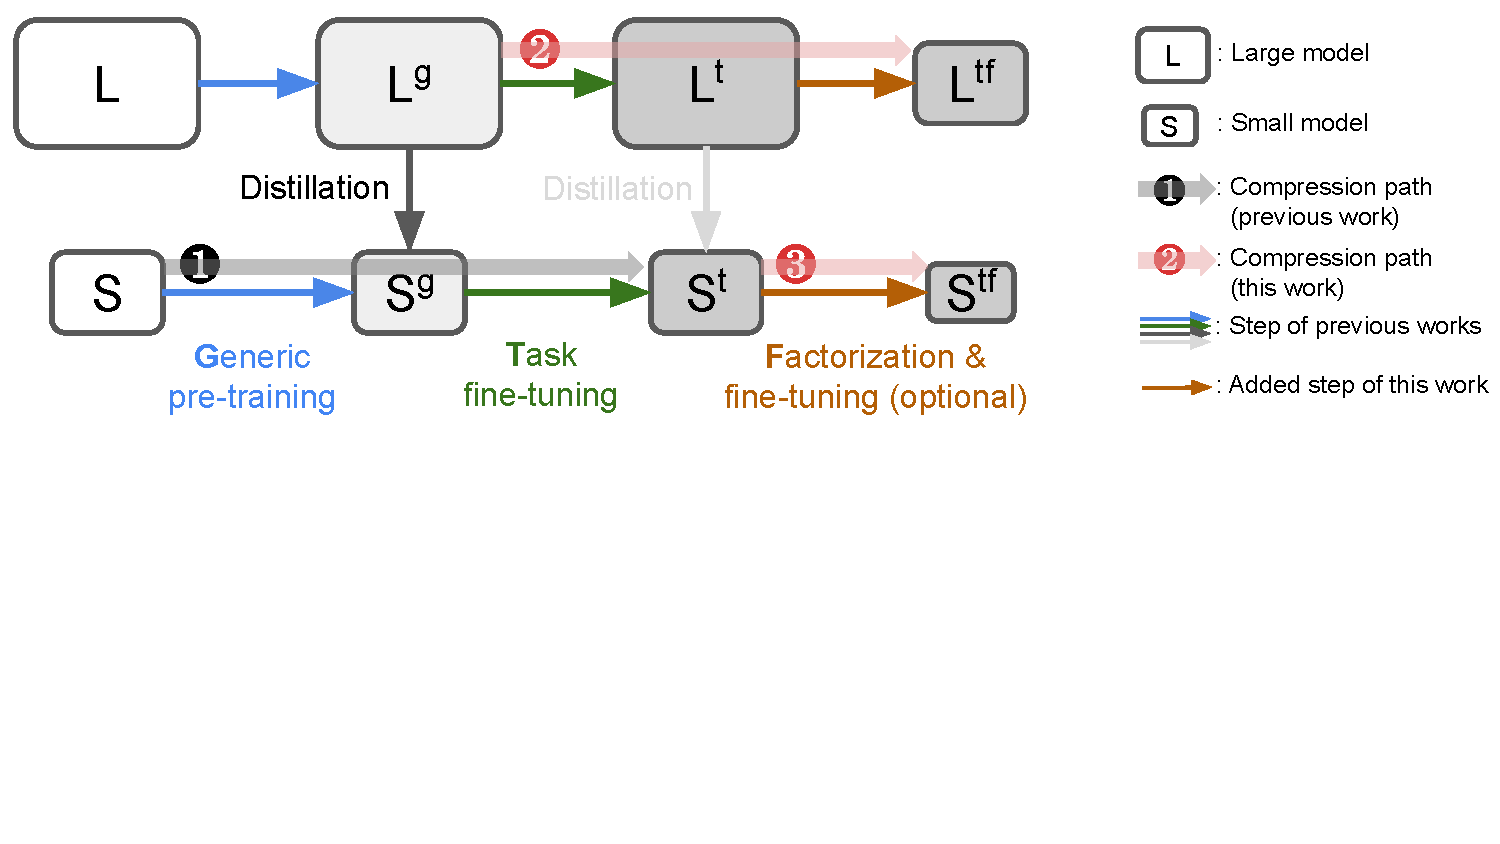
\includegraphics[clip, trim=0cm 7.2cm 0cm 0.3cm, width=0.9\textwidth]{figures/scheme.pdf} 
  \caption{The three paths to create compressed language models are examined in this paper.
  $L/S$ denote the initial models, $L^g/S^g$ are models after generic pre-training,
  $L^t/S^t$ correspond to task-specific models,
  and $L^{tf}/S^{tf}$ are factorized task-specific models. Detailed elaborations are in Sections \ref{sec:3path} nad \ref{sec:3path_implement}
  }\label{fig:scheme}
\end{figure} 

\subsection{Experiment setup}

\subsubsection{Language tasks and datasets}

We evaluate the methods of all three paths in Figure \ref{fig:scheme} on the General Language
Understanding Evaluation (GLUE) benchmark \citep{wang2019glue} and a token classification task.
We include 2 single sentence tasks: CoLA \citep{warstadt2018neural} measured in Matthew's correlation, SST2 \citep{socher2013recursive} measured in classification accuracy; 3 sentence similarity tasks: MRPC \citep{dolan2005microsoft} measured in F-1 score, STS-B \citep{cer-etal-2017-semeval} measured in Pearson-Spearman correlation, QQP \citep{chen2018quora} measured in F-1 score; and 3 natural
language inference tasks: MNLI \citep{williams2018broad} measured in classification accuracy with the average of the matched and mismatched subsets, QNLI \citep{rajpurkar2016squad} measured in accuracy. The token classification task we used is the named entity recognition (NER) on the CoNLL-2003 dataset \citep{sang2003introduction}. In summary, our evaluation includes 8 different natural language tasks.

% We compare our method with a few state-of-the-art pre-BERT model on the General Language Understanding and Evaluation (GLUE) \needcite  benchmark and NER task CoNLL-03. 
% Details of the datasets are shown in Appendix \needcite

\begin{table}%[!tbp]
\centering
\caption{Results of CoNLL and GLUE benchmark. G-Avg means the average of GLUE tasks, A-Avg denotes the average of all tasks, including CoNLL.
Our FWSVD+fine-tuning is the best performer in terms of both average scores,  without the expensive generic pre-training required by path-1 models (e.g., DistillBERT costs 720 V100 GPU hours for training). 
}
\label{tab:GLUE}
\renewcommand\tabcolsep{2.0pt}
\resizebox{1\textwidth}{!}{
\begin{tabular}
%{p{2.3cm}|c|p{0.7cm}p{0.7cm}p{0.7cm}p{0.7cm}p{0.7cm}p{0.7cm}p{0.7cm}p{0.7cm}p{0.7cm}|p{0.7cm}}
{l|l|c|c|ccccccc|c|c}
\toprule
&Model& \#Param &  CoNLL &  CoLA &  MNLI &  MRPC &  QNLI &  QQP  &  SST-2 &  STS-B &  G-Avg & A-Avg \\ \midrule
Original&BERT$_{base}$ & 109.5M & 94.1 & 56.2 & 84.7 & 87.4 & 91.3 & 87.8 & 93.0 & 88.5 & 84.1 & 85.4 \\ \midrule
\multirow{ 2}{*}{Path-1}&DistilBERT & 67.0M & 93.2 & 49.8 & 82.2 & 88.7 & 89.3 & 86.7 & 90.4 & 86.1 & 81.9 & 83.3 \\
&MiniLMv2 & 67.0M & 92.2 & 43.3 & 84.0 & 89.1 & 90.6 & 86.7 & 91.4 & 88.1 & 81.9 & 83.2  \\ \midrule
\multirow{ 5}{*}{Path-2}&BERT-PKD & 67.0M & $-$ & 45.5 & 81.3 & 85.7 & 88.4 & 88.4 & 91.3 & 86.2 & 81.0 & $-$ \\ 
&BERT+SVD & 66.5M & 12.0 & 2.7 & 35.6 & 61.4 & 37.2 & 60.0 & 76.7 & 26.8 & 42.9 & 39.0 \\
&\multicolumn{1}{r|}{+fine-tuning} 
& 66.5M & 92.4 & 40.5 & 82.8 & 84.1 & 89.6 & 87.3 & 90.9 & 85.7 & 80.1 & 81.6 \\
&BERT+FWSVD & 66.5M & 49.6 & 13.5 & 52.8 & 81.2 & 52.2 & 65.7 & 82.1 & 68.6 & 59.4 & 58.2 \\
&\multicolumn{1}{r|}{+fine-tuning} & 66.5M & 93.2 & 49.4 & 83.0 & 88.0 & 89.5 & 87.6 & 91.2 & 87.0 & \textbf{82.2} & \textbf{83.6} \\
\bottomrule
\end{tabular}
}
\end{table}


\subsubsection{Implementation details and the baseline models}\label{sec:3path_implement}

First of all, we use the same training configuration for all the experiments in this paper and avoid any hyperparameter screening to ensure a fair comparison. 

For the SOTA models on path-1 (MiniLMv2 and DistilBERT), we use the pre-trained generic compact models ($S^g$) provided by the original authors as the starting point, then directly fine-tune them with 3 epochs on the target task training data. The fine-tuning is optimized by Adam with learning rate of $2 \times 10^{-5}$ and batch size of 32 on one GPU.

For the methods on path-2 (FWSVD and SVD), we start from the pre-trained generic large model ($L^g$), which is the standard 12-layer BERT model \citep{devlin2018bert}. Then we fine-tune it with the training setting exactly the same as we used for the path-1 models to get the large task-specific models ($L^t$). The last step is applying the low-rank factorization (SVD or FWSVD) followed by another fine-tuning with the same training setting described above. The performance with and without fine-tuning will be both reported.
We also note that we compress only the linear layers in the transformer blocks by reserving only 33\% of the ranks in this work. The setup intentionally makes a fair comparison to the path-1 methods. In other words, we do not compress the non-transformer modules such as the token embedding. Previous works \citep{chen2018groupreduce} have shown significant success in using low-rank factorization to compress the embedding layer, which occupies 23.4M (21.3\%) parameters in the standard BERT model. Therefore, the results we reported for the path-2 methods still have room for improvement by applying our method to non-transformer modules. Lastly, we add BERT-PKD \citep{sun2019patient} based on its reproduced results \citep{chen2018groupreduce} for comparison. BERT-PKD uses knowledge distillation instead of factorization in the path-2 process.

% \yh{talk about the simplification of row-based importance}

For the path-3 experiments, we use the pre-trained task-specific \textit{compact} models ($S^t$) as the starting point. These pre-trained models have a much smaller size (TinyBERT-STSB, MiniLM-CoNLL, MobileBERT-MNLI) or a better performance (DistilBERT-MRPC) than the models we used in the path-1 and path-2, indicating they may contain denser knowledge in their compact models. Therefore, compressing these models introduces a significant challenge. In order to have better coverage for all tasks, we additionally use ALBERT$_{large}$ and ALBERT$_{base}$ \citep{lan2019albert} as the already compact models to generate all 8 task-specific models ($S^g \rightarrow S^t$). Then follow path-3 to compress the compact models. All the training involved here has the same setting as described in path-1.

Lastly, our implementation and experiments are built on top of the popular HuggingFace Transformers library \citep{wolf-etal-2020-transformers}. All other unspecified training settings use the default configuration of the library. Since no hyperparameter tuning is involved in our experiments, we directly report the results on the dev set of all the datasets, making the numbers convenient to compare and verify.

% \subsubsection{Baselines}



\subsection{Path-1 versus Path-2}\label{sec:path1_vs_path2}
%A. BERT+WSVD with finetune (path 2 Vs path 1):
%A1 2nd best avg GLUE 
%A2 stable. no obvious drop. DistilBERT good at COLA, poor at RTE; MiniLMv2 good at RTE but bad at COLA.
Table \ref{tab:GLUE} reports the results of the GLUE benchmark and a NER task. 
Our FWSVD with fine-tuning achieves an average score of $83.6$, beating all other path-1 and path-2 methods.
This is a non-trivial accomplishment since FWSVD with fine-tuning does not need the expensive generic pre-training.
Furthermore, FWSVD has consistent performance retention for all the tasks; it contrasts the path-1 methods, which may have a more considerable variance.
For example, DistilBERT is good at CoLA but poor at STS-B; oppositely,
MiniLMv2 is a strong performer at STS-B but is weak with CoLA. 
In contrast, FWSVD+fine-tuning does not show an obvious shortcoming.


\begin{table}%[!tbp]
\centering
\caption{Results of compressing an already compact model. The original task-specific models are directly downloaded from \href{https://huggingface.co/models}{Huggingface pretrained models}. Our FWSVD successfully reduces more parameters from all the compact models, while achieving the same level of accuracy. (ft: fine-tuning) \vspace{-0.3cm}}
\label{tab:compact}
% \renewcommand\tabcolsep{2.0pt}
\resizebox{1\textwidth}{!}{
\begin{tabular}{l|c|c||c|cccc}\toprule
\multicolumn{3}{c||}{Original Compact Model ($S^t$)} & \multicolumn{5}{c}{Path-3 Compression ($S^t \rightarrow S^{tf}$)} \\ \midrule
Model-Task & \#Param. & Perf. & \#Param. & SVD & SVD+ft. & FWSVD & FWSVD+ft. \\\midrule
TinyBERT-STSB & 14.4M (7.8x) & 87.5 & 11.8M (-18\%) & 73.8 & 86.1 & 84.9 & \textbf{88.0} \\
MiniLM-CoNLL & 22.7M (4.8x) & 88.5 & 18.4M (-19\%) & 12.5 & 88.0 & 70.1 & \textbf{88.6} \\
MobileBERT-MNLI & 24.6M (4.4x) & \textbf{83.6} & 22.5M (-9\%) & 36.4 & 81.9 & 51.1 & 82.5 \\
DistillBERT-MRPC & 66.9M (1.6x) & 88.7 & 46.7M (-30\%) & 0.0 & 83.4 & 67.9 & \textbf{89.0} \\
\bottomrule
\end{tabular}
}
\end{table}
\begin{table}%[!tbp]
\centering
\caption{Results of compressing an already compact model. This table compresses ALBERT \citep{lan2019albert}, which uses the parameter-sharing strategy to create the compact model. FWSVD preserves the performance significantly better than SVD in all 8 tasks, indicating its excellent compatibility in combining the parameter-sharing strategy. This experiment examines the path-3 process.
}
\label{tab:GLUE_albert}
\renewcommand\tabcolsep{2.1pt}
\resizebox{1\textwidth}{!}{
\begin{tabular}
%{p{2.3cm}|c|p{0.7cm}p{0.7cm}p{0.7cm}p{0.7cm}p{0.7cm}p{0.7cm}p{0.7cm}p{0.7cm}p{0.7cm}|p{0.7cm}}
{l|c|c|ccccccc|c|c}
\toprule
Model& \#Param &  CoNLL &  CoLA &  MNLI &  MRPC &  QNLI &  QQP  &  SST-2 &  STS-B &  G-Avg & A-Avg \\ \midrule
BERT$_{base}$ & 109.5M & 94.1 & 56.2 & 84.7 & 87.4 & 91.3 & 87.8 & 93.0 & 88.5 & 84.1 & 85.4 \\ \midrule
ALBERT$_{large}$ & 17.7M & 93.5 & 50.9 & 84.3 & 89.9 & 91.7 & 86.7 & 90.7 & 90.1 & 83.5 & 84.7 \\ \cmidrule{2-12}
\hspace{0.1 in} w SVD & 15.2M (-14\%) & 0.3 & 0.0 & 41.1 & 0.0 & 54.2 & 5.4 & 70.2 & 9.6 & 25.8 & 22.6 \\
\hspace{0.1 in} w SVD+ft. & 15.2M (-14\%) & 92.2 & 46.4 & 83.4 & 81.8 & 49.5 & 86.9 & 89.8 & 86.8 & 74.9 & 77.1 \\
\hspace{0.1 in} w FWSVD & 15.2M (-14\%) & 22.8 & 0.0 & 65.2 & 50.0 & 78.2 & 72.6 & 81.4 & 76.4 & 60.5 & 55.8 \\
\hspace{0.1 in} w FWSVD+ft. & 15.2M (-14\%) & 93.0 & 50.6 & 83.3 & 90.4 & 90.6 & 87.0 & 90.6 & 89.0 & \textbf{83.1} & \textbf{84.3} \\
\midrule
ALBERT$_{base}$ & 11.7M & 92.1 & 43.0 & 82.3 & 88.6 & 90.6 & 86.6 & 89.7 & 89.1 & 81.4 & 82.7 \\ \cmidrule{2-12}
\hspace{0.1 in} w SVD & 9.6M (-18\%) & 3.5 & 0.0 & 32.0 & 0.0 & 55.1 & 53.4 & 52.4 & 9.6 & 28.9 & 25.7 \\
\hspace{0.1 in} w SVD+ft. & 9.6M (-18\%) & 89.8 & 28.8 & 81.3 & 81.2 & 88.3 & 85.5 & 88.2 & 75.0 & 75.5 & 77.3 \\
\hspace{0.1 in} w FWSVD & 9.6M (-18\%) & 16.9 & 6.9 & 55.6 & 47.7 & 69.1 & 54.7 & 72.9 & 54.0 & 51.6 & 47.2 \\
\hspace{0.1 in} w FWSVD+ft. & 9.6M (-18\%) & 91.2 & 42.2 & 81.8 & 86.9 & 88.9 & 86.2 & 88.7 & 87.0 & \textbf{80.2} & \textbf{81.6} \\
\bottomrule
\end{tabular}
}
\end{table}

\subsection{Compressing an already compact model}\label{sec:path3}
%1.our method further compress light-weight models up to 30\% 
%TinyBERT 18.8%, MimiLM 19.2%, Mobile BERT 8% Distill bert 30.4%
%2. even better than TinyBERT with an extreme small size of 11.8M
%3.SVD complete fails in DistillBERT-MRPC
%*. explanation, we only found pretrained models in these tasks. 
The setting of path-3 targets to further compress the lightweight models.
This is challenging as the compact models are already 1.6x $\sim$ 7.8x smaller than the original BERT. 
The results in Table \ref{tab:compact} demonstrate the effectiveness of FWSVD on further reducing the number of parameters. 
The original SVD is almost useless without fine-tuning, while our FWSVD can still retain a significant part of the performance.
For example, SVD ends with a zero accuracy when compressing DistillBERT, while our FWSVD keeps a score of $67.9$ under the same setting.
When combined with fine-tuning, FWSVD can cut off 30\% redundancy for DistillBERT. Even for the highly compact model TinyBERT (only $14.4$M parameters),
FWSVD+fine-tuning still successfully reduces 18\% of the parameters without any performance loss. 
More interestingly, the TinyBERT, MiniLM, and DistillBERT-MRPC compressed by FWSVD+fine-tuning exceed the original performance slightly. The result suggests FWSVD+fine-tuning might introduce a small regularization effect to improve the model's generalizability. 

Lastly, Table \ref{tab:GLUE_albert} examines the compatibility between SVD/FWSVD and the parameter-sharing strategy of the ALBERT model. The average score of ALBERT-large is 84.7\%. The performance of FWSVD (84.3\%) is far better than that of SVD (77.1\%) when both reducing 14\% parameters, suggesting FWSVD is more robust than SVD in combining the parameter-sharing strategy.  



% \subsection{Limitations and future works}
\begin{figure} %[htbp]
  \begin{subfigure}{.32\textwidth}
   \centering
   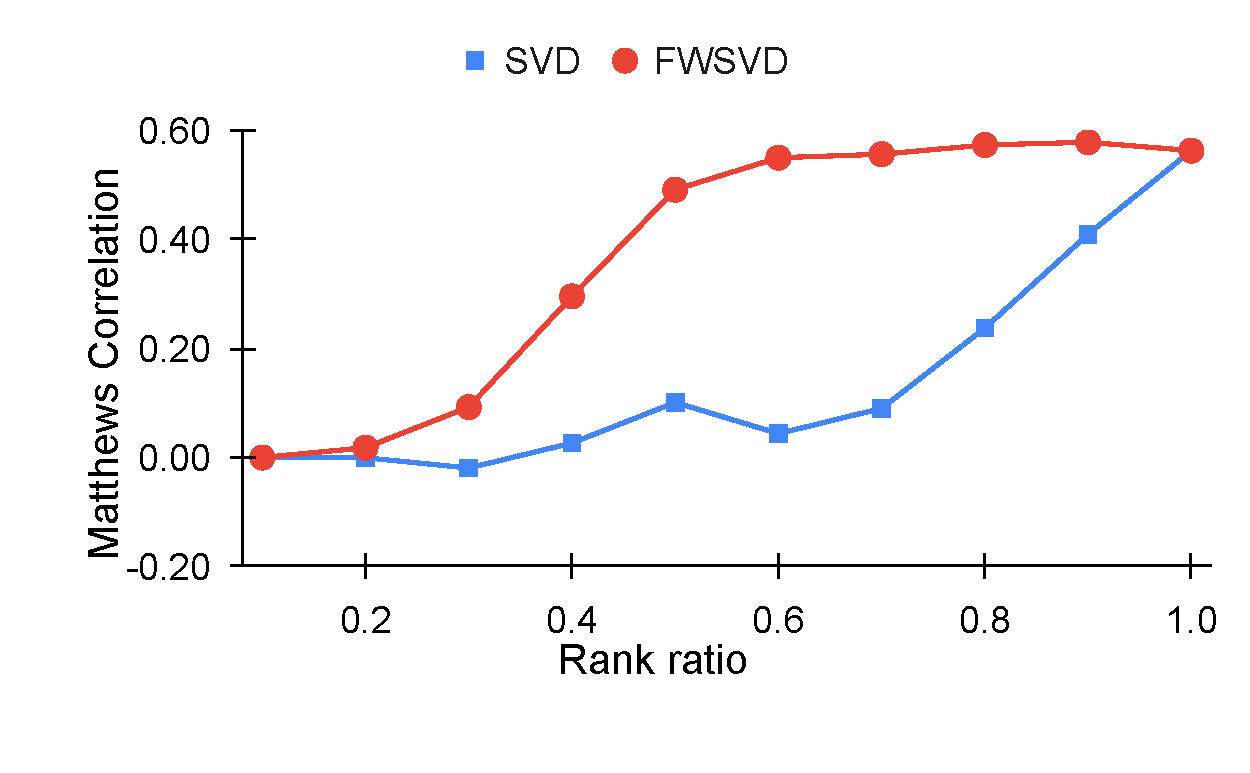
\includegraphics[clip, trim=0cm 0.5cm 0cm 0.5cm,width=\textwidth]{figures/exp_fig1_COLA.pdf}
       \caption{COLA}
       \label{fig:rank:cola}
       \end{subfigure}
\begin{subfigure}{.32\textwidth}
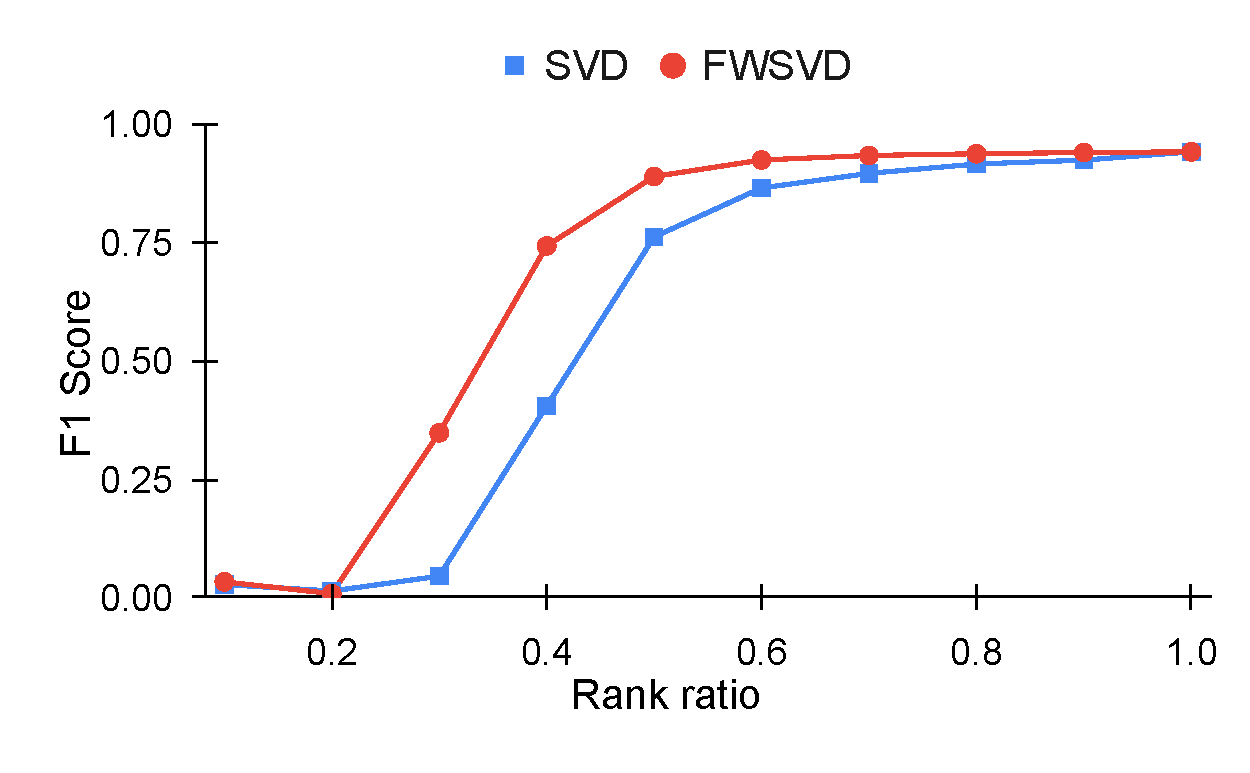
\includegraphics[clip, trim=0cm 0.5cm 0cm 0.5cm,width=\textwidth]{figures/exp_fig1_NER.pdf}
\centering
  \caption{NER (CoNLL-2003)}
   \label{fig:rank:ner}
\end{subfigure}
\begin{subfigure}{.32\textwidth}
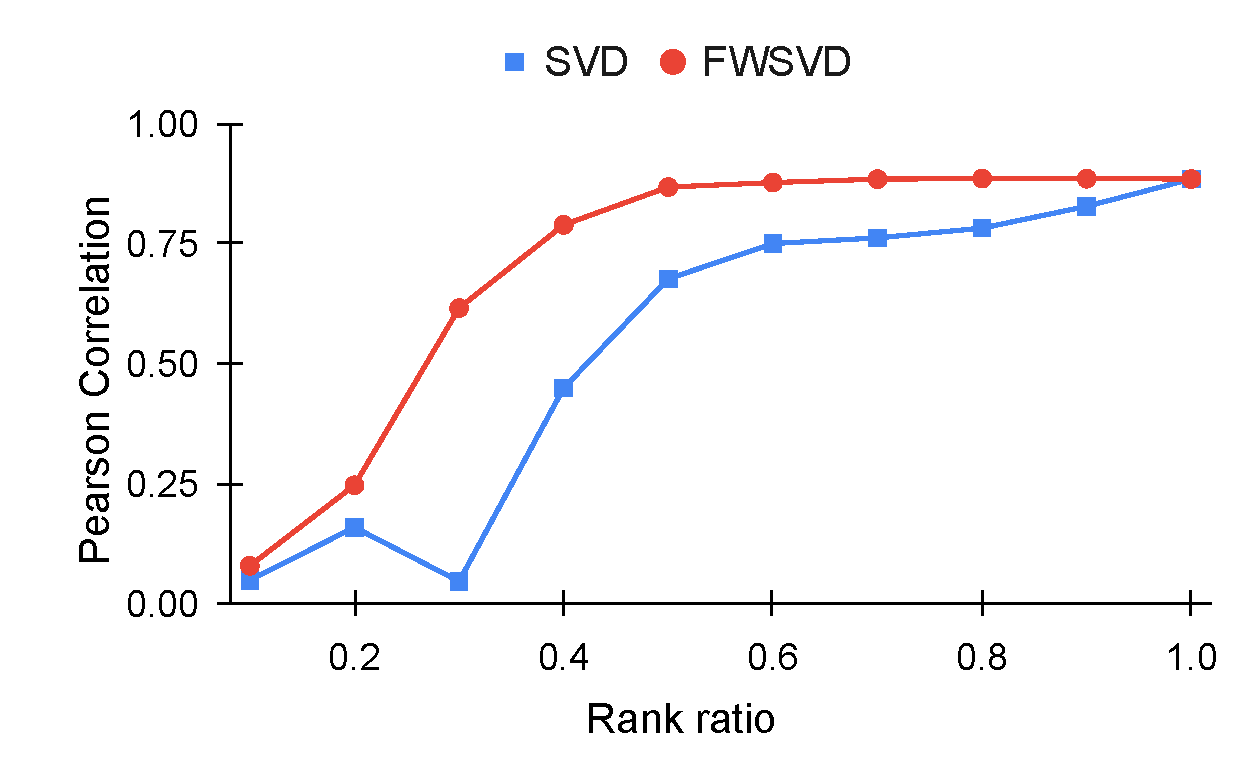
\includegraphics[clip, trim=0cm 0.5cm 0cm 0.5cm,width=\textwidth]{figures/exp_fig1_STSB.pdf}
\centering
  \caption{STS-B}
   \label{fig:rank:stsb}
\end{subfigure}
\caption{FWSVD versus SVD by varying the ratio of reserved ranks. The model with a rank ratio 1.0 indicates the full-rank reconstruction with the same accuracy as the original model (\ie, the $L^t$ in Figure \ref{fig:scheme}). Note that all the models here do not have fine-tuning after factorization. 
% \vspace{-0.3cm}
}
\label{fig:rank}
\end{figure}

\subsection{FWSVD versus SVD}\label{sec:wsvd_vs_svd}

% \subsubsection{Intra path-2 comparison}
%B. SVD Vs WSVD (path 2 alone)
%B1 overall WSVD improves SVD over 26.7\%
%B2 SVD completely fails CoNLL CoLA STS-B. WSVD is 3 to 6 times better
In Table \ref{tab:GLUE}, FWSVD consistently produces much better results than SVD on all tasks. 
On average, FWSVD without fine-tuning obtains an absolute improvement of 17.5\% over SVD. 
To highlight, FWSVD without fine-tuning can maintain a significant portion of performance in challenging tasks such as CoNLL and STS-B, where SVD completely fails. 
With fine-tuning, FWSVD provides better initialization for fine-tuning and consistently achieves a better or comparable performance.

Figure \ref{fig:rank} plots the performance trend with respect to the change of targeted rank ratio, where the full-rank reconstruction corresponds to the results at rank ratio $1.0$.
These results demonstrate the apparent advantage of FWSVD over standard SVD. 
First, at each rank ratio, FWSVD shows significant improvements over SVD. 
Second, the performance of FWSVD keeps growing with the increase of rank ratio, while SVD shows fluctuations in its trend. 
Specifically, two tasks (COLA and STS-B) in Figure \ref{fig:rank} show that SVD has abrupt performance drops at some points. 
On the STS-B task, the performance of SVD at rank ratio $0.3$ is significantly lower than having a smaller rank ratio of $0.2$.
In contrast, FWSVD shows a much stable trend of increasing performance along with the rank ratio.
% \textbf{Why this mismatch between rank ratio and performance happens to SVD while our WSVD is immune to the negative effects?}

\begin{figure}%[htbp]
  \begin{subfigure}[b]{.49\textwidth}
   \centering
   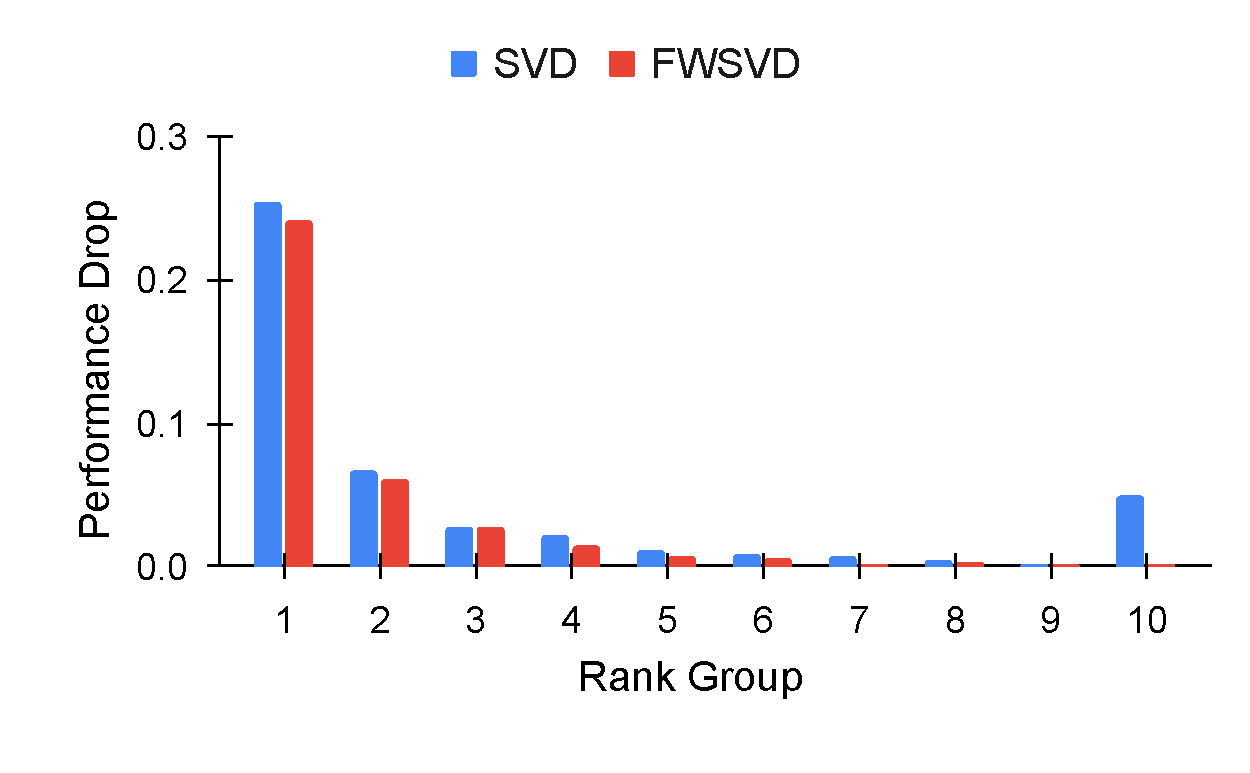
\includegraphics[clip, trim=0cm 0.5cm 0cm 0.5cm, width=\textwidth]{figures/exp_fig2_per_recolor.pdf}
       \caption{STS-B performance drop}
       \label{fig:remove_group:drop}
       \end{subfigure}
\begin{subfigure}[b]{.49\textwidth}
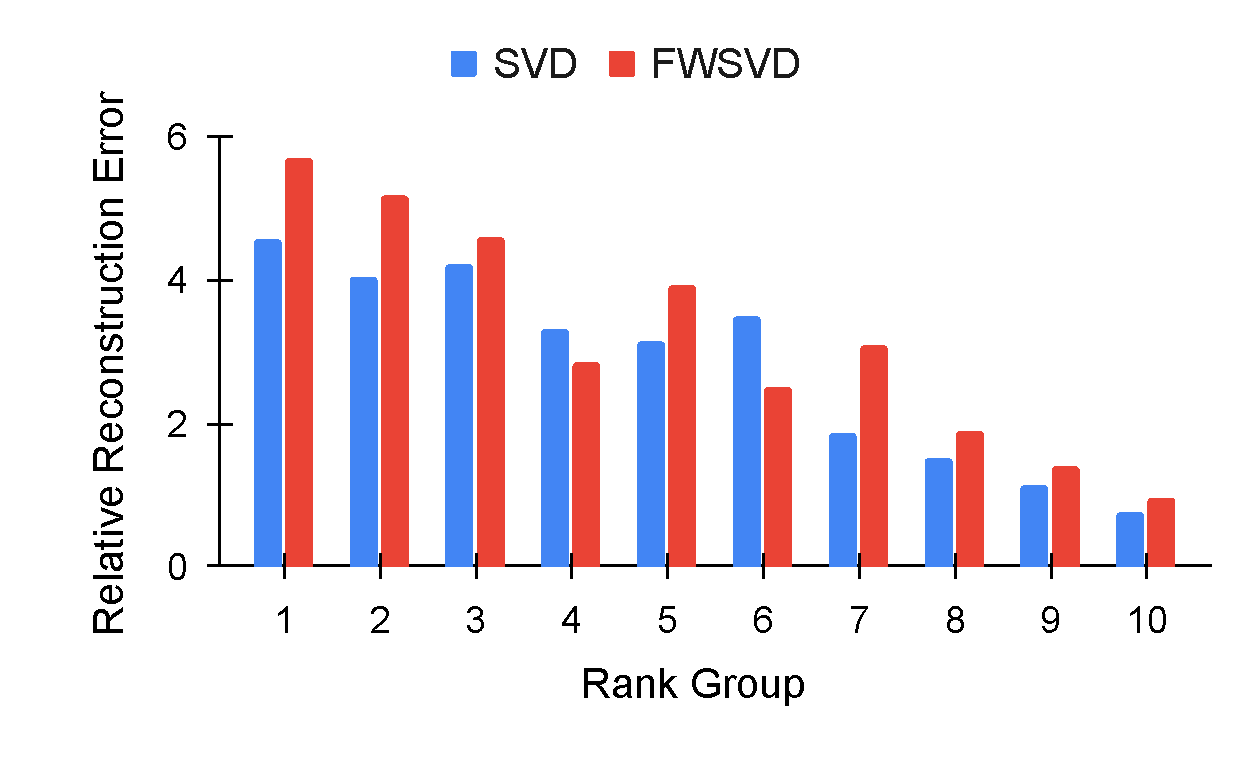
\includegraphics[clip, trim=0cm 0.5cm 0cm 0.5cm, width=\textwidth]{figures/exp_fig2_err_recolor.pdf}
\centering
  \caption{ STS-B reconstruction error}
   \label{fig:remove_group:error}
\end{subfigure}
\caption{
Results of grouped rank truncation on STS-B task. 
% More comparisons on other tasks are presented in Figure \ref{app:err_per} in Appendix.  
In (a), FWSVD shows a consistent trend of having less performance drop with the small singular value groups (group 10 has the smallest singular values), mitigating the issue of Figure \ref{fig:method_rank}. In (b), FWSVD results in a larger reconstruction error with almost all truncated groups, although FWSVD retains the model accuracy better than SVD.
% Unlike SVD, the performance drop of our FWSVD perfectly imitates the ideal trending shown in Figure \ref{fig:method_rank}. 
% \vspace{-0.5cm}
}
\label{fig:remove_group}
\end{figure}

\subsubsection{Revisit the brute force attack }\label{sec:mismatch_obj}

This section applies the same analysis of Section \ref{sec:mismatch}, but adds FWSVD to see if it matches the task's objective better. In Figure \ref{fig:remove_group:drop}, the red bars are significantly lower than the blue bars, especially for the tail groups, which will be truncated first.
We specifically highlight group-10 in \ref{fig:remove_group:drop}, which has the smallest 10\% singular values. The height of the blue bar is equivalent to the size of the overlapped (green and meshed orange) region in Figures \ref{fig:svd}. Similarly, its red bar (close to zero) is equivalent to the overlapped region in Figure \ref{fig:wsvd}. In other words, the illustrations of Figures \ref{fig:svd} and \ref{fig:wsvd} are strongly supported by the results here. Although FWSVD shows a smaller performance drop shown by Figure \ref{fig:remove_group:drop}, it has a more significant reconstruction error than SVD in many cases (see Figure \ref{fig:remove_group:error}), especially with the rank groups that will be truncated first (\eg, groups 5 to 10). In other words, FWSVD's objective (Equation \ref{equ:weight_svd_diag}) aligns with the task objective better by sacrificing the reconstruction error.

% The empirical evidence of mismatched objectives between  a standard low-rank factorization and task performance. The groups with a large performance drop in (a) are equivalent to the green regions in Figure \ref{fig:svd}.

%results:
%A1) top ranks significantly impact the performance
%A2) WSVD  continually decrease
%A3)tail ranks SVD still have strong impact
%B1) SVD always has smaller errors, still more performance loss
%B2) error decrease with group id
%B3) The last group analysis 
% Given a certain targeted rank, standard SVD will discard the ``tail'' singular values in order to achieve the least reconstruction error.
% \textbf{Is it always a wise decision towards the better performance?}


% To study this problem,  we designed the following experiments. First, we split singular values into $r/m$ rank groups by descending order.
% As shown in Equation \ref{equ:gi}, each rank group $g_i$ contains $m$ singular values. 
% We remove one rank group $g_i$ at a time by setting $g_i$ to be a zero vector,
% and this operation will generate a singular values vector $\bar \Sigma_i$.
% Then the ``cripple'' matrix ${{\bar W}_i}$ recomposed by the remaining groups excluded $g_i$ can be computed as follows:
% \begin{equation}
%     {{\bar W}_i} = U \cdot diag({{\bar \Sigma }_i}) \cdot {V^T}.
%     \label{equ:rank_matrix}
% \end{equation}

% We evaluate the performance drop and reconstruction error of the matrix ${{\bar W}_i}$, compared to the full-rank matrix. 
% Taking STS-B taks for example, we split singular values into 10 rank groups, and plot the performance drop and reconstruction errors in Figure \ref{fig:remove_group}.
% As clearly shown in Figure \ref{fig:remove_group}, at each position, although SVD has  the smaller reconstruction errors, FWSVD always enjoys the smaller performance drop. 
%First, as expected by Equation \ref{equ:rank_decomposition}, the top group of singular values has a dominant impact towards the overall performance. \ting{change }
%As shown in Figure \ref{fig:remove_group:drop}, if the first group of  singular values are set zero, the Pearson correlation of STS-B will drop from $0.89$ to around $0.25$ for both SVD and WSVD.
% Figure \ref{fig:remove_group:error} shows the elimination of the top ranked singular values will result in larger reconstruction errors for both FWSVD and SVD. 
% However, when it comes to performance drop, the behaviors of FWSVD and SVD are quite different. 
% For FWSVD, removing a low-ranked group will always cost less performance drop. But this is not true for SVD. 
% With SVD, the removal of Group 10 surprisingly causes a performance drop as large as Group 2.  
% These results prove that lower reconstruction error can not guarantee the better performance.
% And compared to SVD, our proposed FWSVD can better balance the trade-off between the goals of overall performance and reconstruction error. 
% \ting{following table is optional to add} 

% \begin{table}
\centering
\caption{Average absolute reconstruction error of Group-9 and Group-10 in Figure \ref{fig:remove_group}.}
\begin{tabular}{l|cc|cc}
\toprule
{Average absolute }& \multicolumn{2}{c|}{Group-9} & \multicolumn{2}{c}{Group-10} \\ \cline{2-5}
 reconstruction error & SVD & WSVD & SVD & WSVD \\ \midrule
Whole matrix $\bar W$ & 1.34E-05 & 1.59E-05 & 7.77E-06 & 9.55E-06 \\
Top fisher columns $\bar W_f$ & 1.54E-05 & 4.75E-07 & 1.41E-05 & 2.19E-07 \\
\bottomrule
\end{tabular}
\end{table}


% \subsection{Main Results}
